\section{Auswertung}

\subsection{Eckige Stäbe, einseitige Einspannung}

Um den Elastizitätsmodul von den eckigen Stäben bei einseitiger Einspannung zu bestimmen wird zunächst eine Grafik erstellt. Dafür wird die Gesamtauslenkung der eckigen Stäbe bei einseitiger Einspannung D(x) aus den Tabellen \ref{tab:1} und \ref{tab:2} gegen $Lx^2-\frac{x^3}{3}$ aufgetragen. Dabei enstehen folgende Diagramme:

\begin{figure}[H]
    \centering
    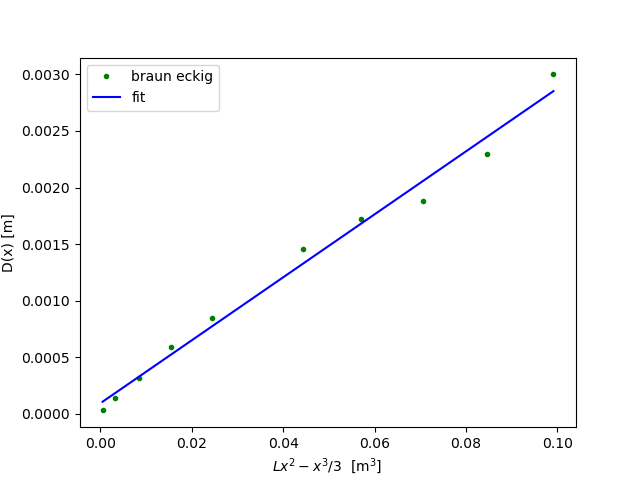
\includegraphics{bee.png}
    \captionof{figure}{Biegung eines braunen, eckigen Stabes mit zugehöriger Ausgleichsrechnung.}
\end{figure}

\begin{figure}[H]
    \centering
    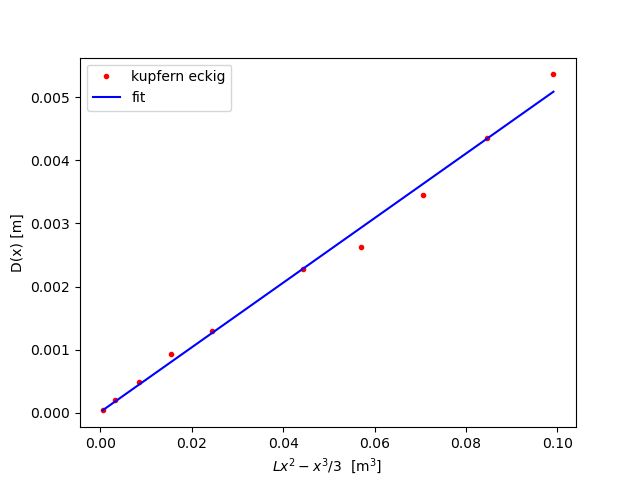
\includegraphics{kee.png}
    \captionof{figure}{Biegung eines kupfernen, eckigen Stabes mit zugehöriger Ausgleichsrechnung.}
\end{figure}

Die Ausgleichsrechnungen wurden mit der allgemeinen Geradengleichung: $y = ax+b$ durchgeführt.
Aus diesen Graphen und den Ausgleichsrechnungen lässt sich der Elastizitätsmodul mit folgender Formel berechnen:

\begin{align*}
    E = \frac{m*g}{2*I*a}
\end{align*}

Dabei ist a die mit der Ausgleichsrechnung bestimmte Steigung der Ausgleichsgeraden.
I ist das Flächenträgheitsmoment. Da die Stäbe Quadratisch sind, ist das Flächenträgheitsmoment: $I=\frac{h^4}{12}$.
Beide Stäbe haben als Kantenlänge h=1cm. Die berechneten Steigungen sind:

\begin{align*}
    a_{braun} = (2.78\pm 0.11) \frac{10^{-2}}{m^2}\\
    a_{kupfern} = (5.1\pm 0.16) \frac{10^{-2}}{m^2} 
\end{align*}

Mit diesen Werten ergibt sich für die Elastizitätsmodule:
\begin{align*}
    E_{braun} = (223\pm 9) GPa \\
    E_{kupfern} = (1.22\pm 4) GPa
\end{align*}

\subsection{runde Stäbe, einseitige Einspannung}

Für die runden Stäbe ist das Vorgehen identisch zu dem Vorgehen bei den Eckigen. Hier werden die Werte von D(x) aus \ref{tab:3} und \ref{tab:4} genommen. Diese werden genauso gegen $Lx^2-\frac{x^3}{3}$ aufgetragen. Dabei entstehen folgende Diagramme:

\begin{figure}[H]
    \centering
    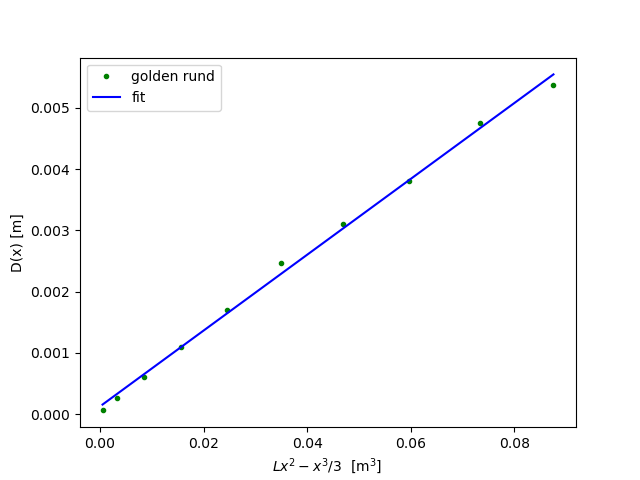
\includegraphics{gre.png}
    \captionof{figure}{Biegung eines goldenen, runden Stabes mit zugehöriger Ausgleichsrechnung.}
\end{figure}

\begin{figure}[H]
    \centering
    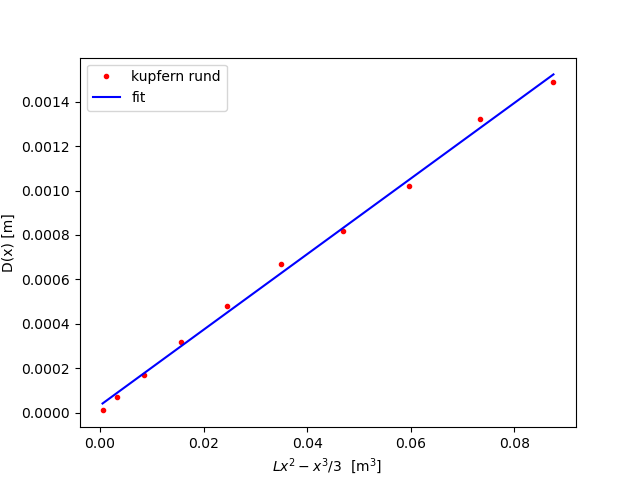
\includegraphics{kre.png}
    \captionof{figure}{Biegung eines kupfernen, runden Stabes mit zugehöriger Ausgleichsrechnung.}
\end{figure}

Auch die Formel für den Elastizitätsmodul bleibt gleich. Der einzige Unterschied ist hier das Flächenträgheitsmoment. Dies lässt sich aufgrund des runden Querschnitts nun folgendermaßen bestimmen:

\begin{align*}
    \frac{\pi R^4}{4}
\end{align*}

Der Durchmesser der beiden Stäbe beträgt 1cm.

Nun lassen sich wieder die Elastizitätsmodule bestimmen:

\begin{align*}
    E_{kupfern} = (146.5\pm 2.6) GPa \\
    E_{golden} = (89\pm 17) GPa 
\end{align*}

\subsection{eckige Stäbe, beidseitige Einspannung}



\section{Messwerte}

\begin{minipage}{\linewidth}
    \begin{table}[H]
        \centering
    \captionof{table}{brauner, eckiger Stab}
    \begin{tabular}{lll}
        \toprule
        x [cm] & D(x) (einseitig) [mm] & D(x) (beidseitig) [mm] \\
        \midrule
        3  & 0.03 & 0.015 \\
        8  & 0.14 & 0.07  \\
        13 & 0.32 & 0.11  \\
        18 & 0.59 & 0.17  \\
        23 & 0.85 & 0.22  \\
        32 & 1.46 & 0.24  \\
        37 & 1.72 & 0.21  \\
        42 & 1.88 & 0.16  \\
        47 & 2.30 & 0.12  \\
        52 & 3.00 & 0.05  \\
        \bottomrule   
    \end{tabular}
    
    \label{tab:1}
\end{table}
\end{minipage}


\begin{minipage}{\linewidth}
    \begin{table}[H]
        \centering
    \captionof{table}{kupferner, eckiger Stab}
    \begin{tabular}{lll}
        \toprule
        x [cm] & D(x) (einseitig) [mm] & D(x) (beidseitig) [mm] \\
        \midrule
        3  & 0.04 & 0.09 \\
        8  & 0.21 & 0.20 \\
        13 & 0.49 & 0.38 \\
        18 & 0.93 & 0.45 \\
        23 & 1.29 & 0.52 \\
        32 & 2.28 & 0.57 \\
        37 & 2.62 & 0.51 \\
        42 & 3.45 & 0.44 \\
        47 & 4.35 & 0.26 \\
        52 & 5.36 & 0.11 \\
        \bottomrule   
    \end{tabular}
    
    \label{tab:2}
\end{table}
\end{minipage}

\begin{minipage}{\linewidth}
    \begin{table}[H]
        \centering
    \captionof{table}{kupferner, runder Stab}
    \begin{tabular}{lll}
        \toprule
        x [cm] & D(x) (einseitig) [mm] & x2 [cm] & D(x) (beidseitig) [mm] \\
        \midrule
        3  & 0.01 & 3  & 0.01 \\ 
        8  & 0.07 & 8  & 0.09 \\ 
        13 & 0.17 & 13 & 0.18 \\ 
        18 & 0.32 & 18 & 0.28 \\ 
        23 & 0.48 & 23 & 0.36 \\ 
        28 & 0.67 & 32 & 0.42 \\ 
        33 & 0.82 & 37 & 0.37 \\ 
        38 & 1.02 & 42 & 0.29 \\ 
        43 & 1.32 & 47 & 0.15 \\ 
        48 & 1.49 & 52 & 0.08 \\ 
        \bottomrule   
    \end{tabular}
    
    \label{tab:3}
\end{table}
\end{minipage}

\begin{minipage}{\linewidth}
    \begin{table}[H]
        \centering
    \captionof{table}{goldener, runder Stab}
    \begin{tabular}{lll}
        \toprule
        x [cm] & D(x) (einseitig) [mm] & x2 [cm] & D(x) (beidseitig) [mm] \\
        \midrule
        3  & 0.06 & 3  & 0.29 \\ 
        8  & 0.26 & 8  & 0.72 \\ 
        13 & 0.61 & 13 & 1.12 \\ 
        18 & 1.10 & 18 & 1.39 \\ 
        23 & 1.70 & 23 & 1.58 \\ 
        28 & 2.46 & 32 & 1.60 \\ 
        33 & 3.1  & 37 & 1.43 \\ 
        38 & 3.8  & 42 & 1.19 \\ 
        43 & 4.75 & 47 & 0.78 \\ 
        48 & 5.37 & 52 & 0.33 \\ 
        \bottomrule   
    \end{tabular}
    
    \label{tab:4}
\end{table}
\end{minipage}